\documentclass[
	12pt,				  % tamanho da fonte
	openright,		% capítulos começam em pág ímpar (insere página vazia caso preciso)
	a4paper,			% tamanho do papel. 
	% -- opções do pacote babel --
	english,			% idioma adicional para hifenização
	french,				% idioma adicional para hifenização
	spanish,			% idioma adicional para hifenização
	brazil,				% o último idioma é o principal do documento
]{abntex2}
\usepackage[acronym]{glossaries}


% PACOTES

% ---
% Pacotes fundamentais 
\usepackage{lmodern}			  % Usa a fonte Latin Modern
\usepackage[T1]{fontenc}		% seleção de códigos de fonte.
\usepackage[utf8]{inputenc} % Codificação do documento (conversão automática dos acentos)
\usepackage{indentfirst}		% Indenta o primeiro parágrafo de cada seção.
\usepackage{color}				  % Controle das cores
\usepackage{graphicx}			  % Inclusão de gráficos
\usepackage{microtype} 			% para melhorias de justificação
% ---

% Pacotes adicionais, usados no anexo do modelo de folha de identificação
\usepackage{multicol}
\usepackage{multirow}

\usepackage{float} % para utilizar o H de tabelas e figuras e mante-las no lugar
% ---
\usepackage{xcolor}
% Definindo novas cores
\definecolor{verde}{rgb}{0,0.5,0}
\usepackage{listings}
\lstset{
  language=Verilog, %indicar a linguagem utilizada
  basicstyle=\ttfamily\tiny, 
  keywordstyle=\color{blue}, 
  stringstyle=\color{verde}, 
  commentstyle=\color{gray}, 
  extendedchars=true, 
  showspaces=false, 
  showstringspaces=false, 
  numbers=left,
  numberstyle=\tiny,
  breaklines=true, 
  backgroundcolor=\color{green!10},
  breakautoindent=true, 
  captionpos=b,
  xleftmargin=0pt,
}

% Pacotes de citações
\usepackage[brazilian,hyperpageref]{backref}	 % Paginas com as citações na bibl
\usepackage[alf]{abntex2cite}	                 % Citações padrão ABNT
\citebrackets()                                % citação numérica entre colchetes
% --- 


% CONFIGURAÇÕES DE PACOTES

% Configurações do pacote backref
% Usado sem a opção hyperpageref de backref
\renewcommand{\backrefpagesname}{Citado na(s) página(s):~}
% Texto padrão antes do número das páginas
\renewcommand{\backref}{}
% Define os textos da citação
\renewcommand*{\backrefalt}[4]{
	\ifcase #1 %
		Nenhuma citação no texto.%
	\or
		Citado na página #2.%
	\else
		Citado #1 vezes nas páginas #2.%
	\fi
}%
% ---


% Informações de dados para CAPA e FOLHA DE ROSTO
\titulo{
	Desenvolvimento e 
	implementação de um processador compatível com a 
	Arquitetura 6502 em FPGA
}
\autor{Wilson Cazarré Sousa} 
\local{São José dos Campos - Brasil}
\data{Abril de 2024}
\instituicao{
  Docente: Prof. Dr. Tiago de Oliveira
  \par
  Universidade Federal de São Paulo - UNIFESP
  \par
  Instituto de Ciência e Tecnologia - Campus São José dos Campos
}
\tipotrabalho{Relatório técnico}
\preambulo{
	Relatório apresentado à Universidade Federal de São Paulo como parte dos
	requisitos para aprovação na disciplina de Laboratório de Sistemas
	Computacionais: Arquitetura e Organização de Computadores.
}
% ---

% Configurações de aparência do PDF final

% alterando o aspecto da cor azul
\definecolor{blue}{RGB}{41,5,195}

% informações do PDF
\makeatletter
\hypersetup{
     	%pagebackref=true,
		pdftitle={\@title}, 
		pdfauthor={\@author},
		pdfsubject={\imprimirpreambulo},
		pdfcreator={LaTeX with abnTeX2},
		pdfkeywords={abnt}{latex}{abntex}{abntex2}{relatório técnico}, 
		colorlinks=true,       		% false: boxed links; true: colored links
		linkcolor=blue,          	% color of internal links
		citecolor=blue,        		% color of links to bibliography
		filecolor=magenta,      		% color of file links
		urlcolor=blue,
		bookmarksdepth=4
}
\makeatother
% --- 


% Espaçamentos entre linhas e parágrafos 

% O tamanho do parágrafo é dado por:
\setlength{\parindent}{1.3cm}

% Controle do espaçamento entre um parágrafo e outro:
\setlength{\parskip}{0.2cm}  % tente também \onelineskip

% compila o indice
\makeindex
% ---

% ----------------------------------------------------------
% GLOSSÁRIO
% ----------------------------------------------------------
\makeglossaries

\newacronym{ab}{BE}{Barramento de Endereços}
\newacronym{db}{BD}{Barramento de Dados}


% ------------------------------------------------
% Início do documento
\begin{document}

% Seleciona o idioma do documento (conforme pacotes do babel)
%\selectlanguage{english}
\selectlanguage{brazil}

% Retira espaço extra obsoleto entre as frases.
\frenchspacing

% ----------------------------------------------------------
% ELEMENTOS PRÉ-TEXTUAIS
% ----------------------------------------------------------
% \pretextual

% ---
% Capa
\imprimircapa
% ---

% ---
% Folha de rosto
\imprimirfolhaderosto*
% ---

% ---
% RESUMO
% resumo na língua vernácula (obrigatório)
\setlength{\absparsep}{18pt} % ajusta o espaçamento dos parágrafos do resumo
\begin{resumo}


	\noindent
	\textbf{Palavras-chaves}: 6502. FPGA. RISC. CISC.
\end{resumo}

%------LISTAS SÃO OPCIONAIS---------
% inserir lista de ilustrações


\pdfbookmark[0]{\listfigurename}{lof}
\listoffigures*
\clearpage

% inserir lista de tabelas
\pdfbookmark[0]{\listtablename}{lot}
\listoftables*
\clearpage
% ---


\printglossary[type=\acronymtype, title=Lista de Abreviações]
\clearpage

%SUMÁRIO É OBRIGATÓRIO
% inserir o sumario
\pdfbookmark[0]{\contentsname}{toc}
\tableofcontents*
% ---


% ----------------------------------------------------------
% ELEMENTOS TEXTUAIS
\textual

% ----------------------------------------------------------
\chapter{Introdução}
Durante a disciplina de Laboratório de Sistemas Computacionais:
Arquitetura e Organização de Computadores ofertada, é proposto que os discentes
escolham um arquitetura para realizar sua implementação em um dispositivo FPGA.
Esse relatório irá apresentar a fundamentação, bem como todo o processo de
desenvolvimento de um sistema computacional baseado no microprocessador 6502.


\section{Motivação}
mandaram eu fazer esse trabalho ou eu seria reprovado na matéria
\section{Metodologia}
ai eu peguei lá o negócio e n sei oq lá ai eu fiz as coisas
com meus manos e no final ficou tudo chave
\section{Organização do relatório}
ao leitor: basta ler
\section{Objetivos}
\subsection*{Geral}
Descrever o objetivo geral do projeto
\subsection*{Específico}
Descrever com detalhes os objetivos da etapa atual.

\chapter{Fundamentação Teórica}

\section{Visão geral de um sistema computacional}
\subsection{Arquitetura de von Neumann}
\subsection{Interfaces de entrada e saída}
\subsection{Microprocessadores}

\section{Microprocessador 6502}

O microprocessador 6502 é o segundo membro da família MCS650X. Essa família de
microprocessadores de 8 bits foi lançada em 1975 pela \emph{MOS Technology}.
Os processadores dessa família apresentam o mesmo conjunto de instruções e modos
de endereçamento, com pequenas diferenças em recursos e sua utilização. Por
conta de sua eficácia e baixo custo, o microprocessador se popularizou
rapidamente ao ser usado em diversos sistemas da época como \emph{O Nintendo
	Entertainment System (NES)}, \emph{Apple II}, \emph{Commodore 64} e muitos
outros.
\subsection{Arquitetura Original}
O microprocessador conta com um \acrfull{db} de 8 bits e um \acrfull{ab} de
16-bits. Qualquer operação que o processador precisa executar normalmente é
iniciada colocando o endereço de acesso no \acrshort{ab} e posteriormente lendo
(ou escrevendo) um valor de 8-bits no \acrshort{db}.

Internamente, 3 registradores de propósito geral podem ser usados.
\begin{itemize}
	\item \textbf{Acumulador (A)}: Usado também para armazenar o resultado das
	      operações lógicas e aritméticas;
	\item \textbf{\emph{Index} X e Y}: Ambos os registradores podem ser usados
	      para operações com modos de endereçamento especiais, que serão abordados
	      mais a frente no relatório.
\end{itemize}

Além dos 3 registradores que podem ser acessados diretamente, o 6502 também
possuí alguns registradores usados por funções específicas do processador.

\subsection{Registrador de Status (SR)}

O \textbf{registrador de status} é responsável por armazenar \emph{flags} usadas
para o controle do fluxo de programa do processador. Elas normalmente são
atualizadas durante operações lógicas, aritméticas e de transferência de dados.
\begin{itemize}
	\item \textbf{\emph{Carry (C)}}: Indica se a operação gerou um \emph{carry};
	\item \textbf{Negativo (N)}: Indica se a operação gerou um valor com o bit
	      mais significativo ativo;
	\item \textbf{\emph{Overflow} (V)}: Indica se a operação gerou um...;
	\item \textbf{Zero (Z)}: Indica se a operação gerou o valor zero;
	\item \textbf{Decimal (D)}: Indica se o processador está em modo aritmético
	      decimal BCD;
	\item \textbf{Bloqueio de interrupções (I)}: Indica se o processador está
	      ignorando as requisição de interrupções;
	\item \textbf{\emph{Break} (B)}: Indica se a interrupção atual foi disparada
	      via \emph{software} pela instrução BRK, ao invés de uma interrupção via
	      \emph{hardware}.
\end{itemize}

\subsection{Contador de Programa (PC)}
O único registrador de 16-bits definido pela arquitetura. Esse registrador é
responsável por manter o endereço de memória atualmente acessado pelo
processador.

\subsection{\emph{Stack Pointer} (SP)}
O \emph{stack} é uma região de memória destinada para rápido acesso e escrita.
A eficácia nessas operações vem do fato de que o processador utiliza o endereço
no SP para saber exatamente onde a próxima leitura e escrita vai ocorrer.
O registrador é incrementado ou decrementado de acordo após cada operação. O
6502 também utiliza o \emph{stack} para armazenar os endereços de retorno quando
subrotinas ou interrupções são executadas.

\subsection{Modos de endereçamento}
O 6502 é capaz de endereçar 65536 bytes de memória. Qualquer operação ou
estrutura de dados dentro do processador compartilham esse mesmo espaço de
memória. O processador também providencia 13 diferentes métodos de calcular o
endereço efetivo de memória na qual a operação vai ser executada. Na computação,
chamamos esses métodos de \textbf{modos de endereçamento} e aqueles disponíveis
no 6502 serão descritos aqui.

\subsubsection{Endereçamento imediato}
Nesse tipo de instrução o operando é usado imediatamente após a instrução ter
sido lida. Nenhum acesso a memória ou cálculo é realizado
(\autoref{fig:address:imm}). Essa tipo de instrução utiliza 2 bytes de memória.

\begin{figure}[h]
	\centering
	\caption{Endereçamento imediato} \label{fig:address:imm}
	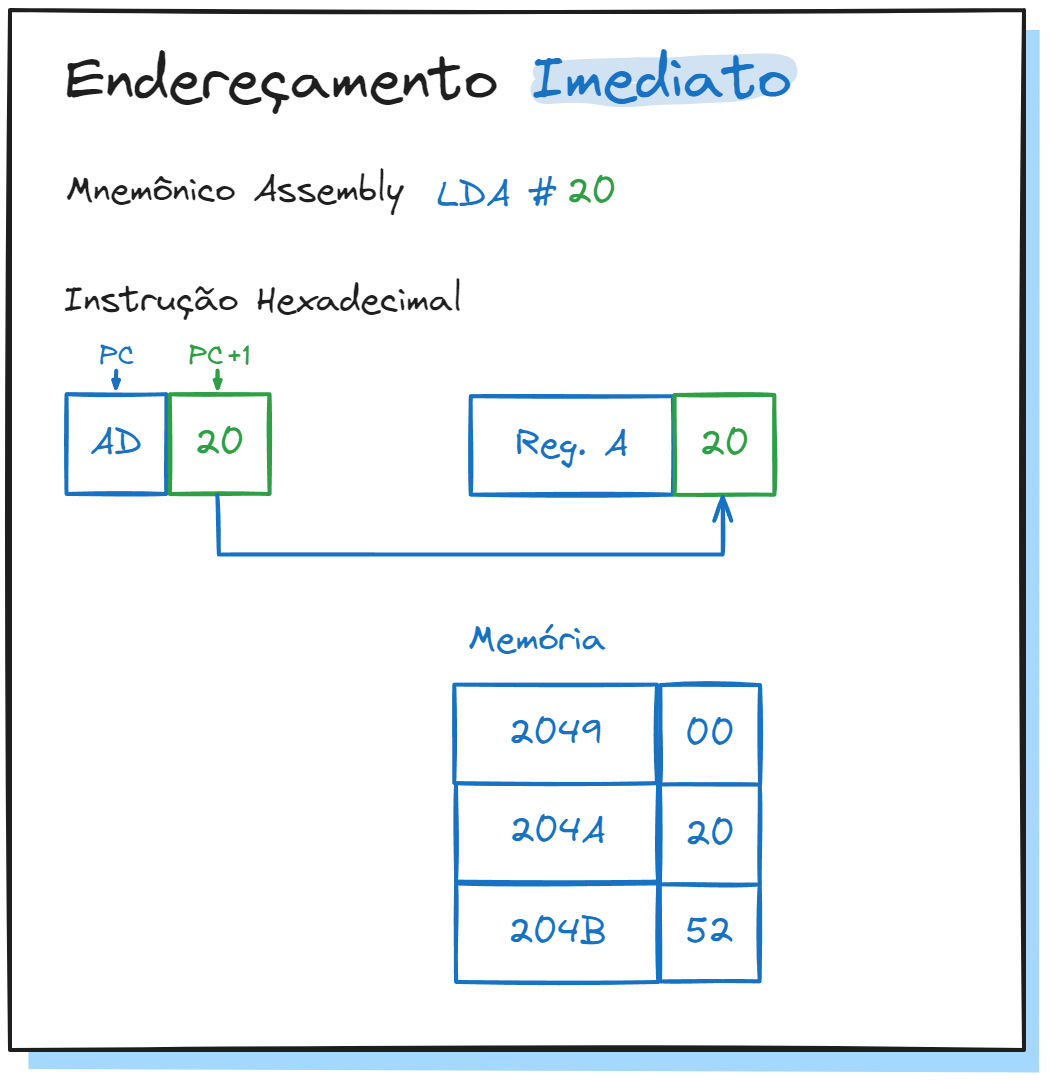
\includegraphics[scale=0.25]{../assets/img/addressing-modes-imm.png}
	\legend{Fonte: Autoria própria}
\end{figure}

\subsubsection{Endereçamento absoluto}
Nesse tipo de instrução dois bytes são passados além do opcode. O processador
usa esses bytes como um endereço de acesso a memória (\autoref{fig:address:abs}).
\begin{figure}[h]
	\centering
	\caption{Endereçamento absoluto. Note que o primeiro byte na memória é o menos
		significativo}
	\label{fig:address:abs}
	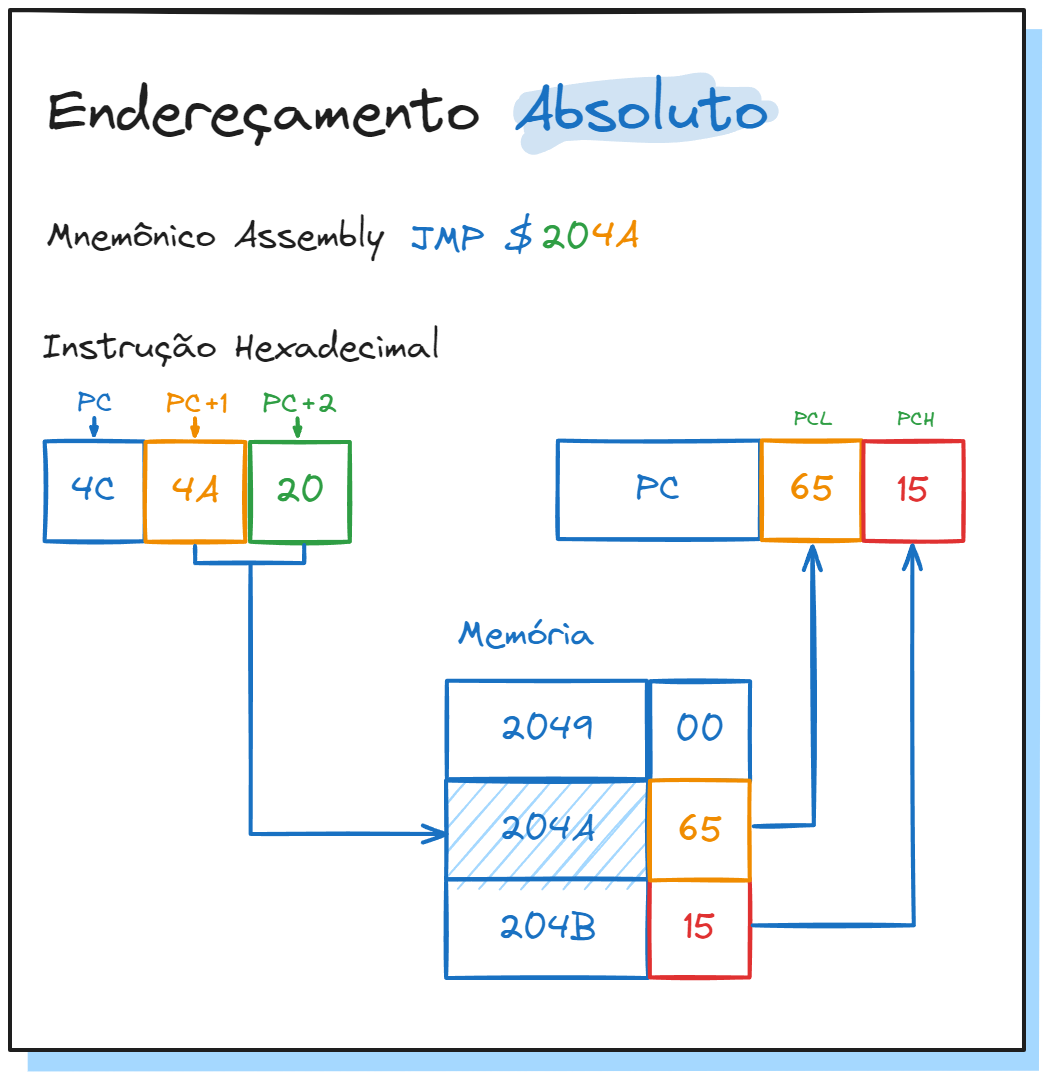
\includegraphics[scale=0.25]{../assets/img/addressing-modes-abs.png}
	\legend{Fonte: Autoria própria}
\end{figure}

\subsubsection{Endereçamento absoluto - Deslocado em X (ou Y)}
Esse modo é uma variação do endereçamento absoluto: dois bytes são buscados da
memória e usados como endereço de acesso. A diferença está no fato de que o
valor do registrador (X ou Y) é somado ao endereço de acesso.
(\autoref{fig:address:absx}).
\begin{figure}[H]
	\centering
	\caption{Endereçamento absoluto - Deslocado em X (ou Y)}
	\label{fig:address:absx}
	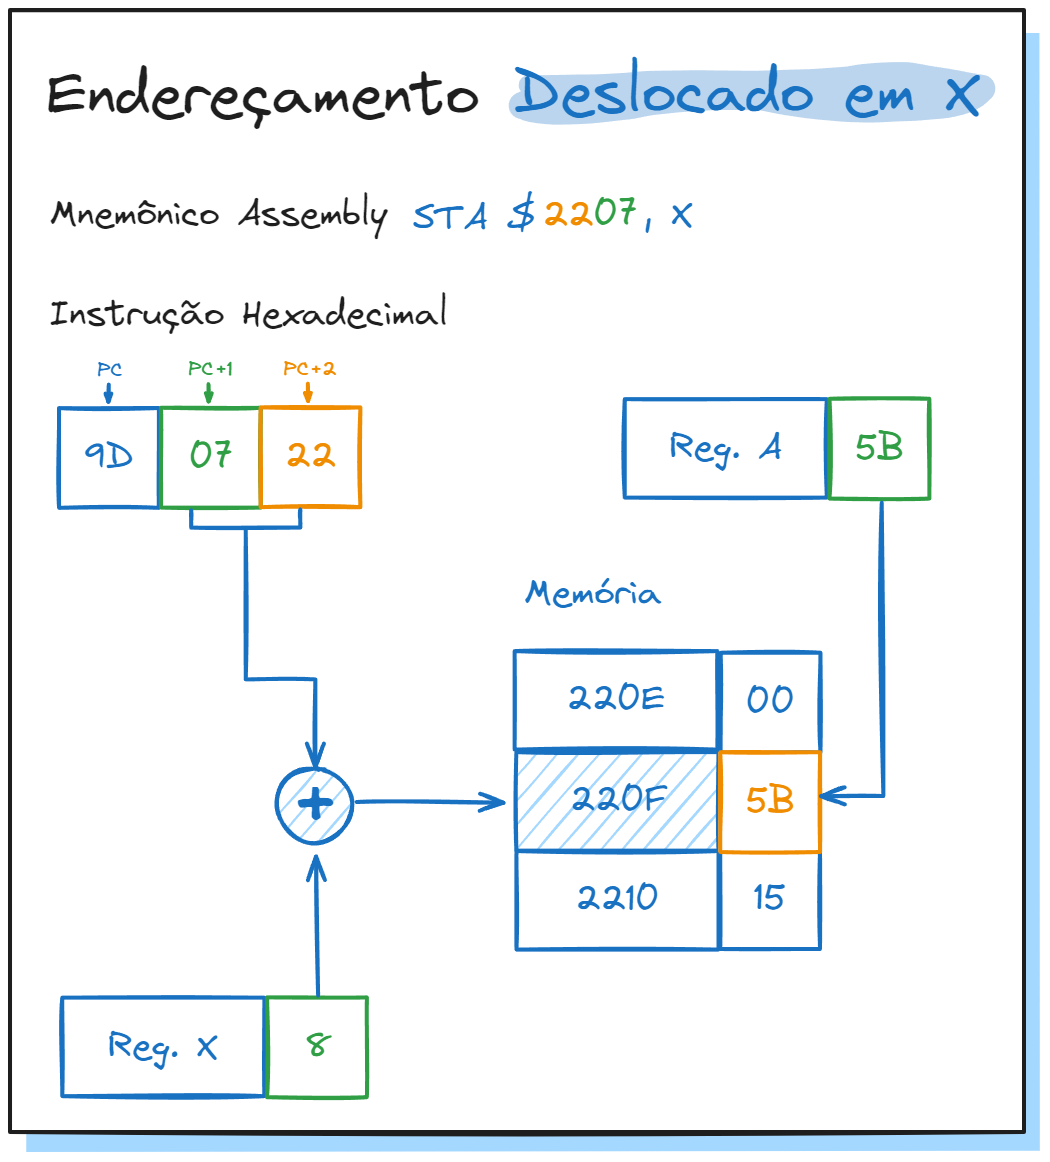
\includegraphics[scale=0.25]{../assets/img/addressing-modes-absx.png}
	\legend{Fonte: Autoria própria}
\end{figure}

\subsubsection{Endereçamento \emph{Zero-Page}}
Idêntico ao endereçamento absoluto, exceto que apenas um byte é lido da memória
(o byte menos significativo). O byte mais significativo é inferido como 0
\autoref{fig:address:zpg}. Logo esse modo de endereçamento sempre retorna um
dado localizado na primeira "página" da memória (os primeiros 256 bytes).
\begin{figure}[h]
	\centering
	\caption{Endereçamento \emph{Zero-Page}} \label{fig:address:zpg}
	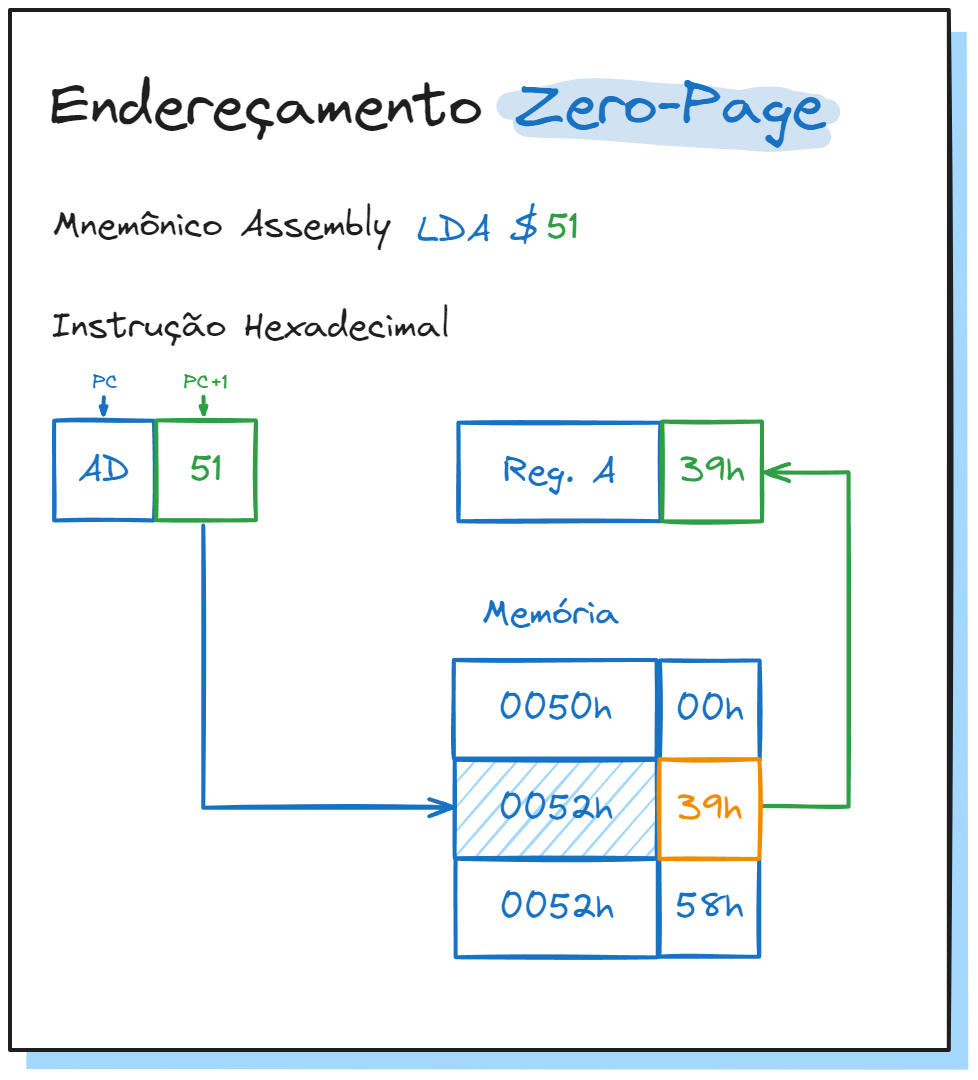
\includegraphics[scale=0.25]{../assets/img/addressing-modes-zpg.png}
	\legend{Fonte: Autoria própria}
\end{figure}

\subsubsection{Endereçamento relativo}
esse tbm
\begin{figure}[H]
	\centering
	\caption{Endereçamento relativo} \label{fig:address:rel}
	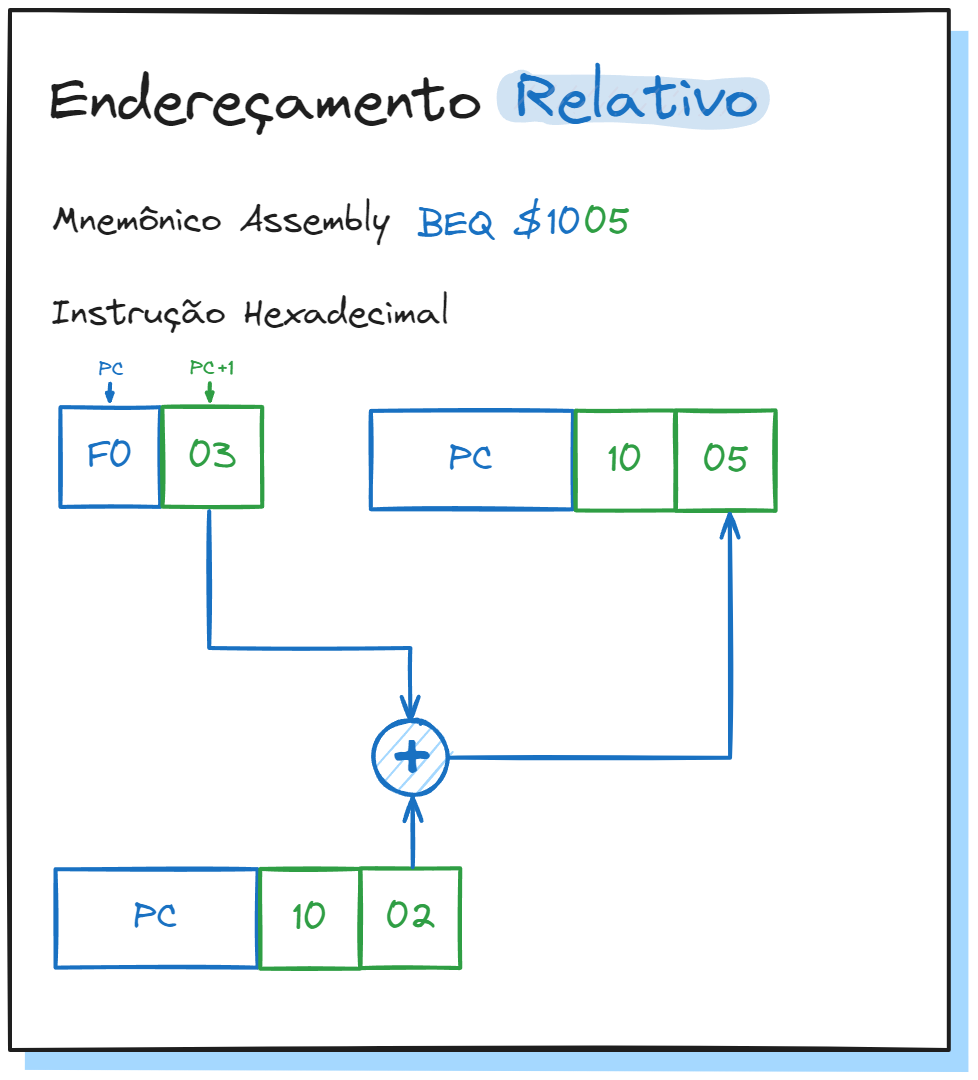
\includegraphics[scale=0.25]{../assets/img/addressing-modes-rel.png}
	\legend{Fonte: Autoria própria}
\end{figure}

\subsubsection{Endereçamento indireto}
\autoref{fig:address:ind}
\begin{figure}[H]
	\centering
	\caption{Endereçamento indireto} \label{fig:address:ind}
	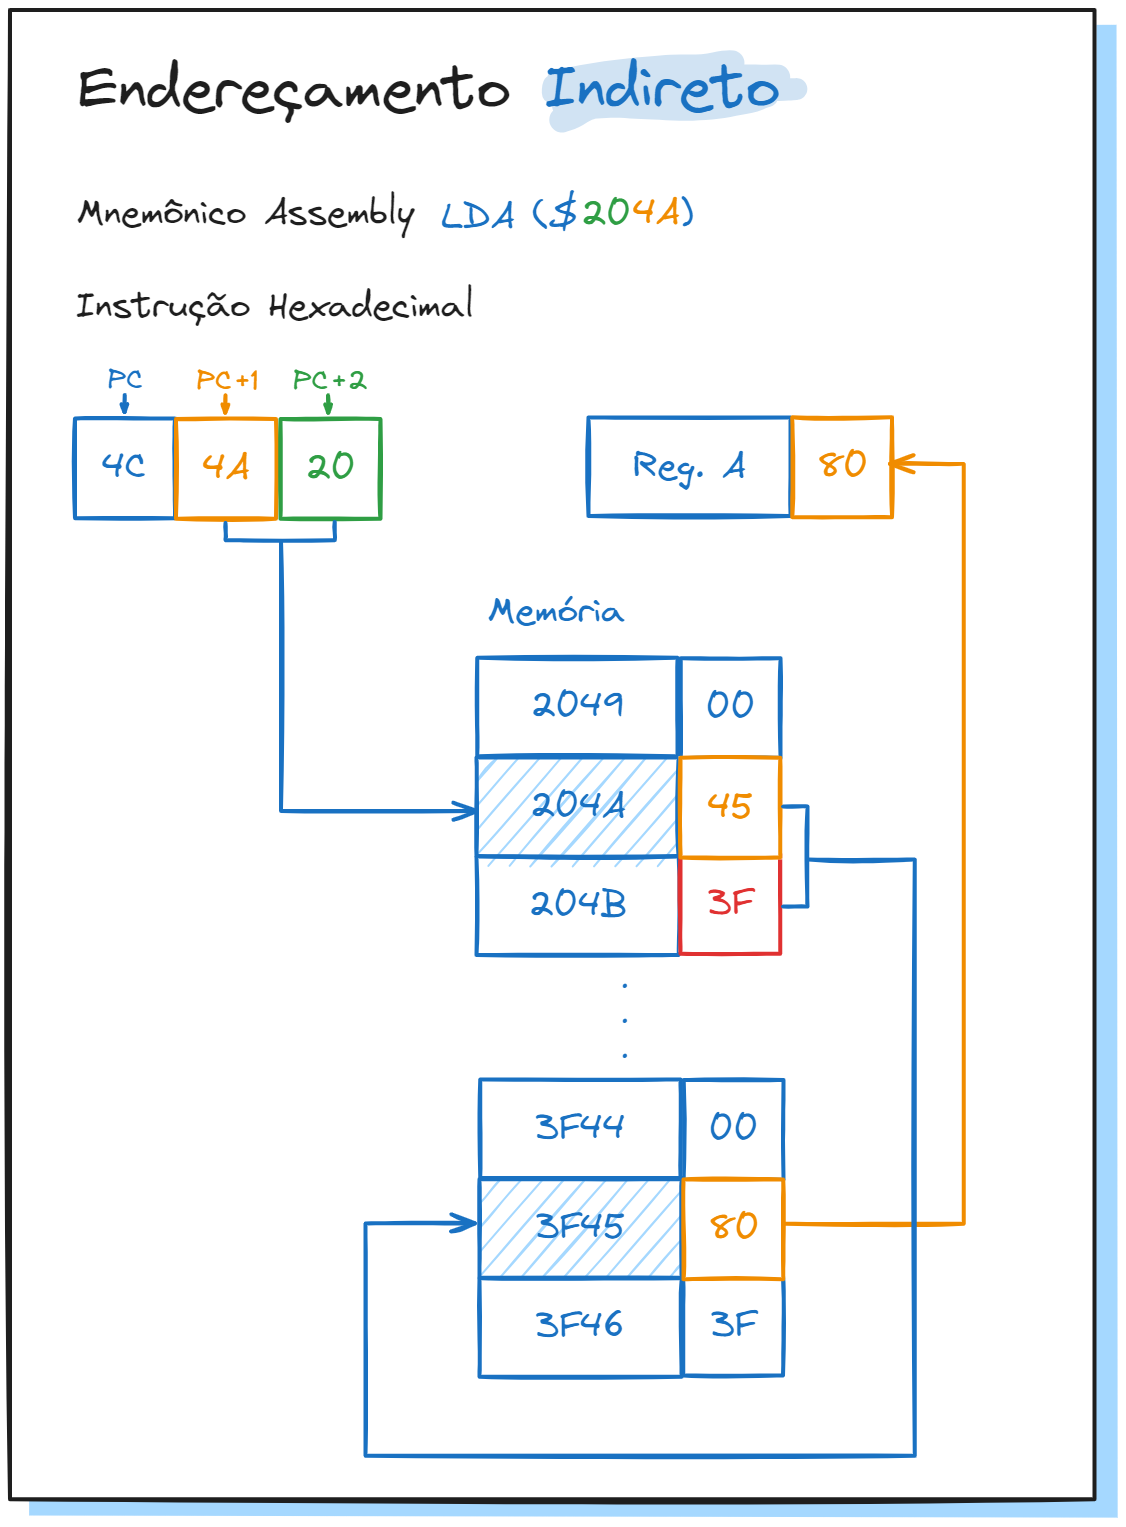
\includegraphics[scale=0.25]{../assets/img/addressing-modes-ind.png}
	\legend{Fonte: Autoria própria}
\end{figure}

\subsection{Endereçamento \emph{Zero-Page}, deslocado em X (ou Y)}
Idêntico ao Endereçamento Absoluto deslocado em X (ou Y) com a diferença que o
endereço de acesso está sempre dentro da primeira

\section{RTL - \emph{Register-Transfer Logic}}
Quando tratamos do design de circuitos digitais complexos, é comum abstrairmos
diferentes níveis do design com a intenção de tornar esses problemas mais
simples de serem resolvidos.

3 níveis diferentes de abstração são definidos por \citeonline{vahid2011} na
construção de circuitos digitais:
\begin{enumerate}
	\item \textbf{\emph{Transistor Level}}: Conectar transistores para construir
	      componentes lógicos.
	\item \textbf{\emph{Logic Level}}: Utilizar-se de Portas Lógicas como bloco
	      principal de construção para desenvolver circuitos combinacionais.
	\item \textbf{\emph{Register-transfer Level}}: Conectar uma rede de
	      registradores e construir blocos que definem a lógica de transferência de
	      estado entre esses registradores.
\end{enumerate}

De maneira geral, no \emph{Register-Transfer Level Design} (ou Design RTL) cada
bloco do design deve desempenhar uma (e apenas uma) de duas possíveis funções:
\begin{enumerate}
	\item \textbf{Lógica Combinacional}: São os blocos responsáveis pela
	      computação do próximo estado. De maneira geral, esses blocos devem ser
	      determinísticos e sempre apresentar a mesma saída para uma determinada
	      entrada.
	\item \textbf{Lógica Sequencial}: São blocos responsáveis por guardar e
	      propagar o estado computado pelos blocos combinacionais de maneira
	      síncrona.
\end{enumerate}

\begin{table}[htb]
	\centering
	\ABNTEXfontereduzida
	\caption{Tamanho da instrução por modo de endereçamento} \label{tab:Instr3OP}
	\begin{tabular}{l|c}
		\textbf{Modo de endereçamento}            & \textbf{Tamanho em bytes} \\ \hline
		Acumulador (A)                            & 1                         \\ \hline
		Absoluto (abs)                            & 3                         \\ \hline
		Absoluto, deslocado em X (abs, x)         & 3                         \\ \hline
		Absoluto, deslocado em Y (abs, y)         & 3                         \\ \hline
		Imediato (\#)                             & 2                         \\ \hline
		Implícito (impl)                          & 1                         \\ \hline
		Indireto (ind)                            & 3                         \\ \hline
		Indireto, deslocado em X (X, ind)         & 2                         \\ \hline
		Indireto, deslocado em Y (ind, Y)         & 2                         \\ \hline
		Relativo (rel)                            & 2                         \\ \hline
		\emph{Zero-Page} (zpg)                    & 2                         \\ \hline
		\emph{Zero-Page}, deslocado em X (zpg, x) & 2                         \\ \hline
		\emph{Zero-Page}, deslocado em Y (zpg, y) & 2                         \\ \hline
	\end{tabular}
	\legend{Fonte: Autoria Própria}
\end{table}


\section{FPGA - Field Programmable Array}

\section{Verilog Sintetizável}

\section{Completude de Turing}

\chapter{Desenvolvimento}

\begin{figure}[H]
	\centering
	\caption{Endereçamento indireto} \label{fig:6502}
	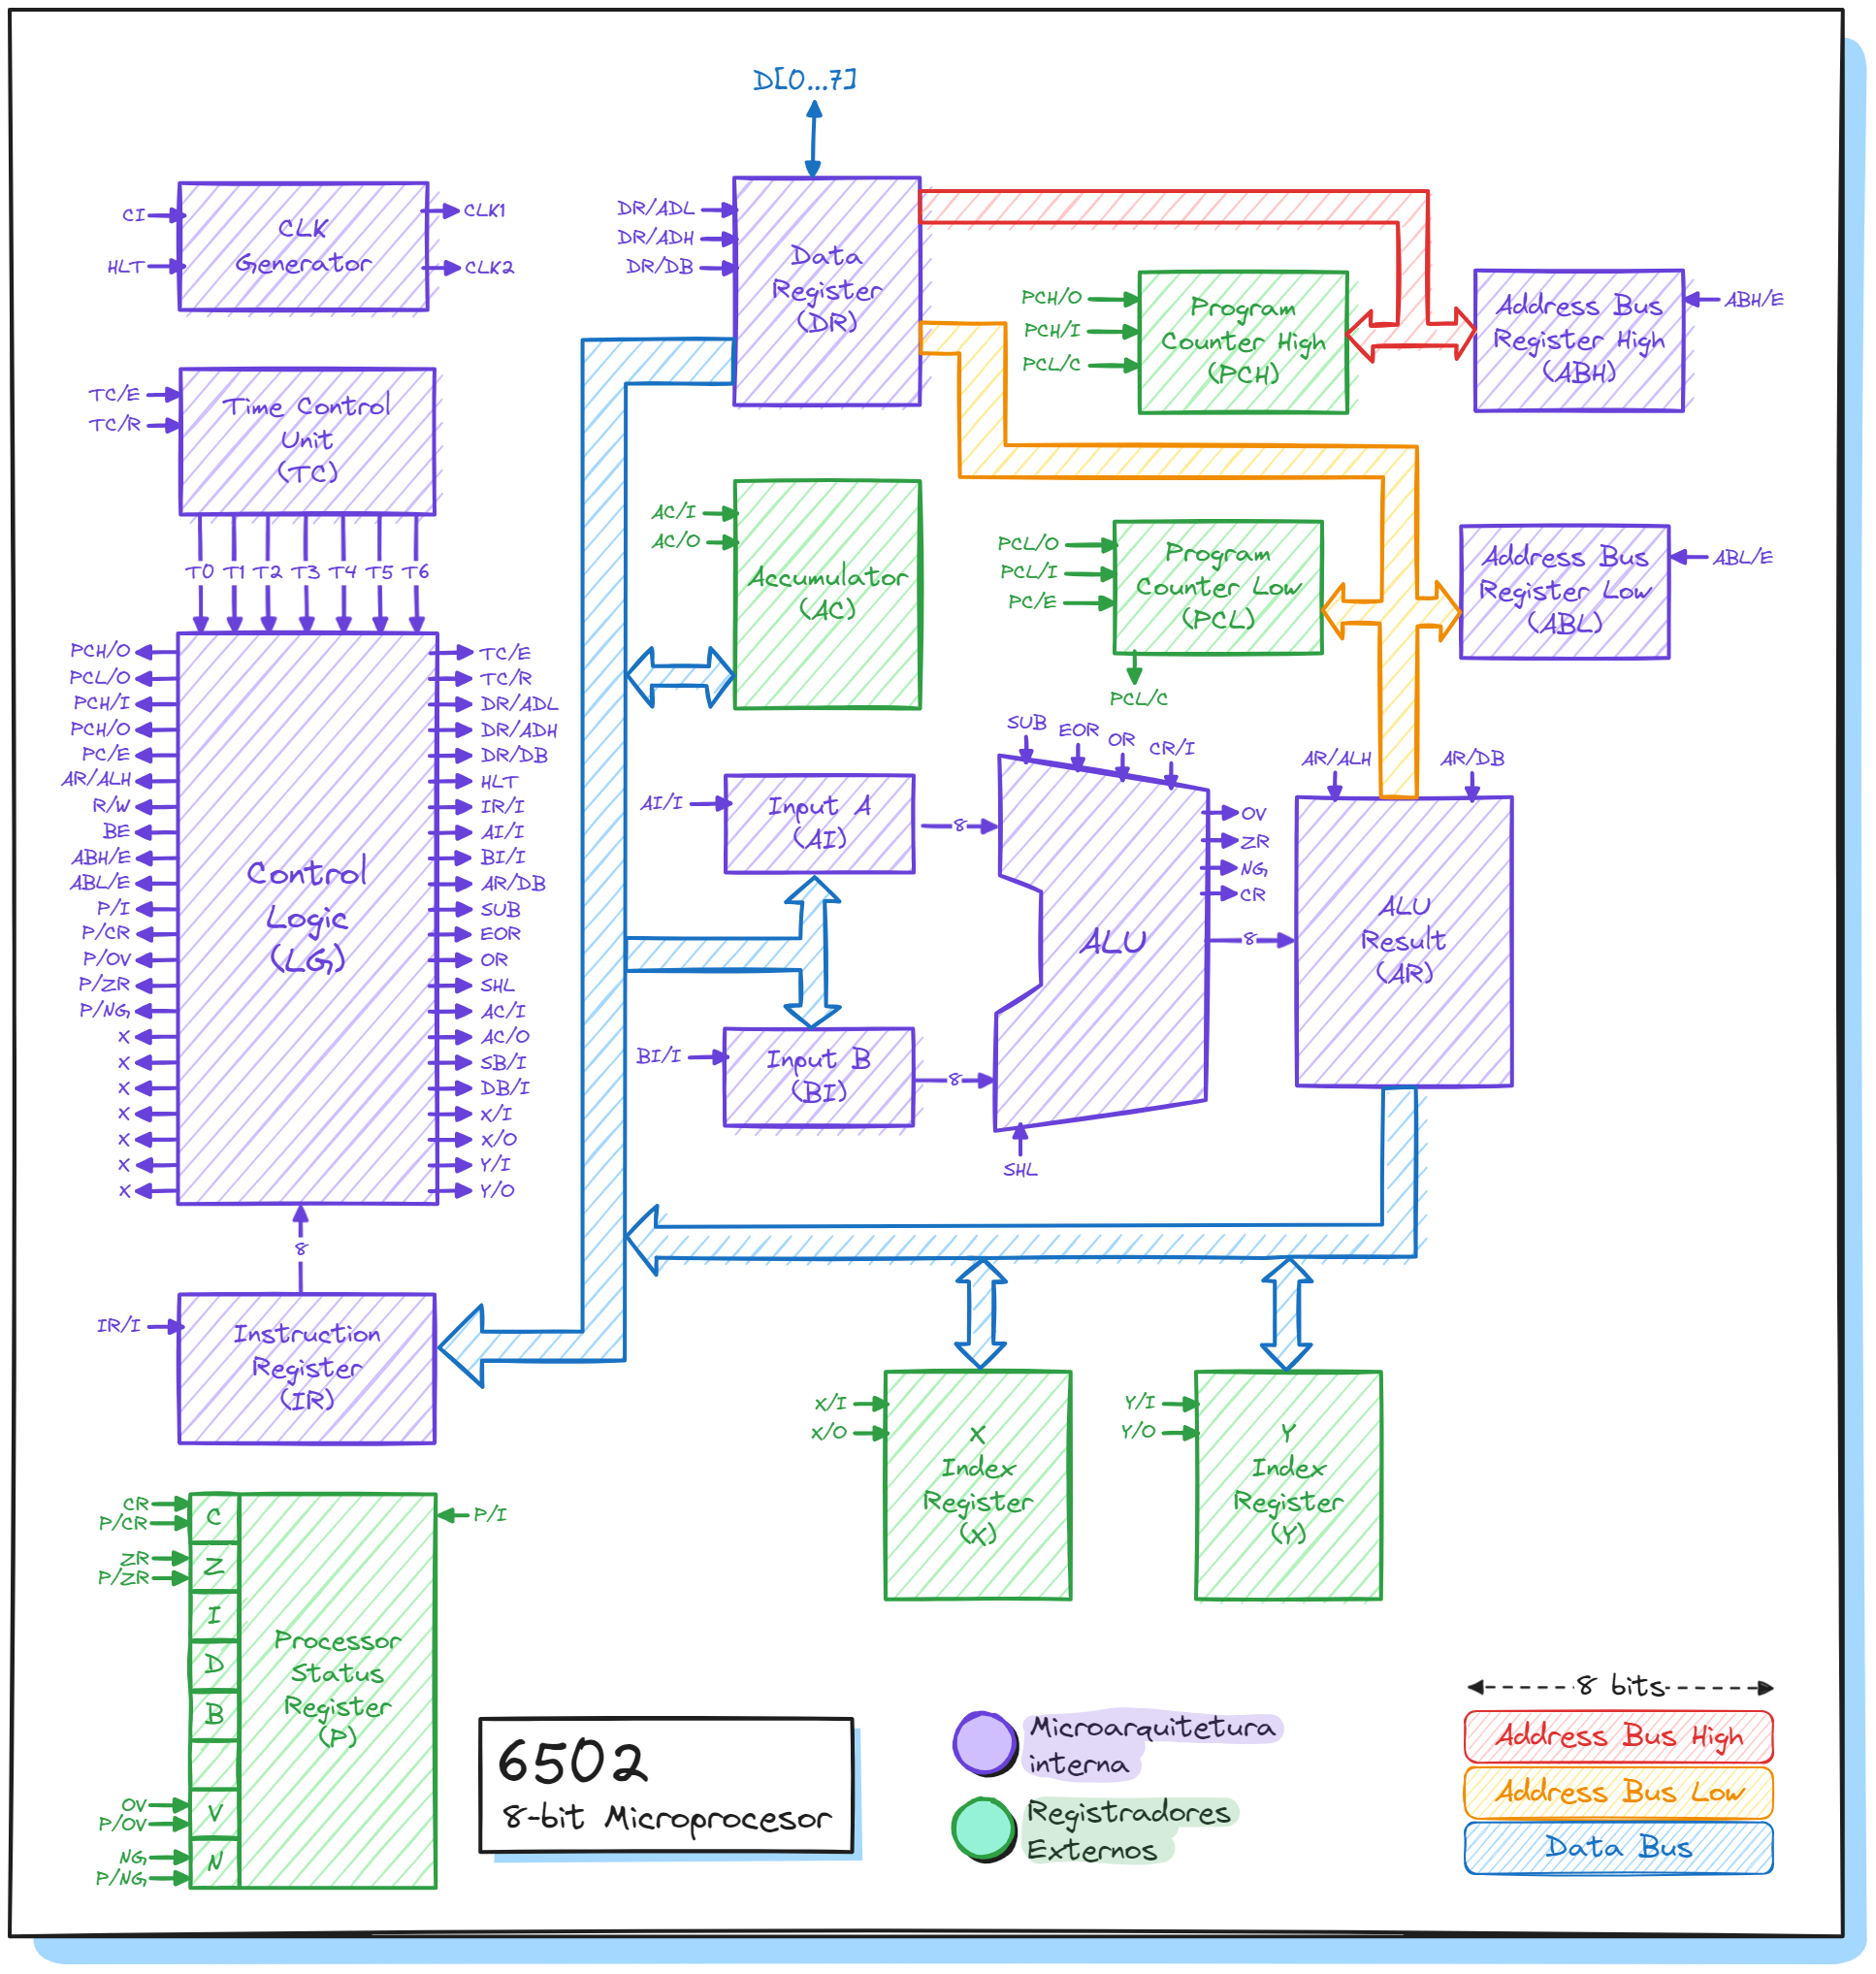
\includegraphics[scale=0.25]{../assets/img/6502.png}
	\legend{Fonte: Autoria própria}
\end{figure}


\section{Unidades funcionais}

\subsection{Registradores}
\begin{itemize}
	\item A
	\item X
	\item Y
	\item SP
	\item PC
	\item SR
\end{itemize}
\subsection{Unidade de Controle}
A unidade de controle é responsável por enviar os sinais de controle para
o processador com o objetivo de executar o comando armazenado no Registrador
de Instruções.


\chapter{Resultados Obtidos e Discussões}


\chapter{Considerações Finais}



% ---
% Finaliza a parte no bookmark do PDF
% para que se inicie o bookmark na raiz
% e adiciona espaço de parte no Sumário
% ---
\phantompart


% ----------------------------------------------------------
% ELEMENTOS PÓS-TEXTUAIS
% ----------------------------------------------------------
\postextual

% ----------------------------------------------------------
% Referências bibliográficas
% ----------------------------------------------------------
\bibliography{referencias}


% ----------------------------------------------------------
% Apêndices
% ----------------------------------------------------------

% ---
% Inicia os apêndices
% ---
\begin{apendicesenv}

	% Imprime uma página indicando o início dos apêndices
	\partapendices

\end{apendicesenv}
% ---


% ----------------------------------------------------------
% Anexos
% ----------------------------------------------------------

% ---
% Inicia os anexos
% ---
\begin{anexosenv}

\end{anexosenv}




\clearpage

%---------------------------------------------------------------------
% INDICE REMISSIVO
%---------------------------------------------------------------------

\phantompart

\printindex

\printglossary
\printglossary[type=\acronymtype, title=Lista de Abreviações]


\end{document}
